\chapter{System Photographs and Dashboard Visuals}
\label{app:screenshots}

\section{Smart Footstep Energy Harvester Prototype}
Figure~\ref{fig:hero_prototype} presents the physical StepCharge AI smart floor tile prototype, demonstrating the integration of piezoelectric transducers with the impact distribution plate.

\begin{figure}[H]
\centering
\IfFileExists{figures/stepcharge-hero.jpg}{
    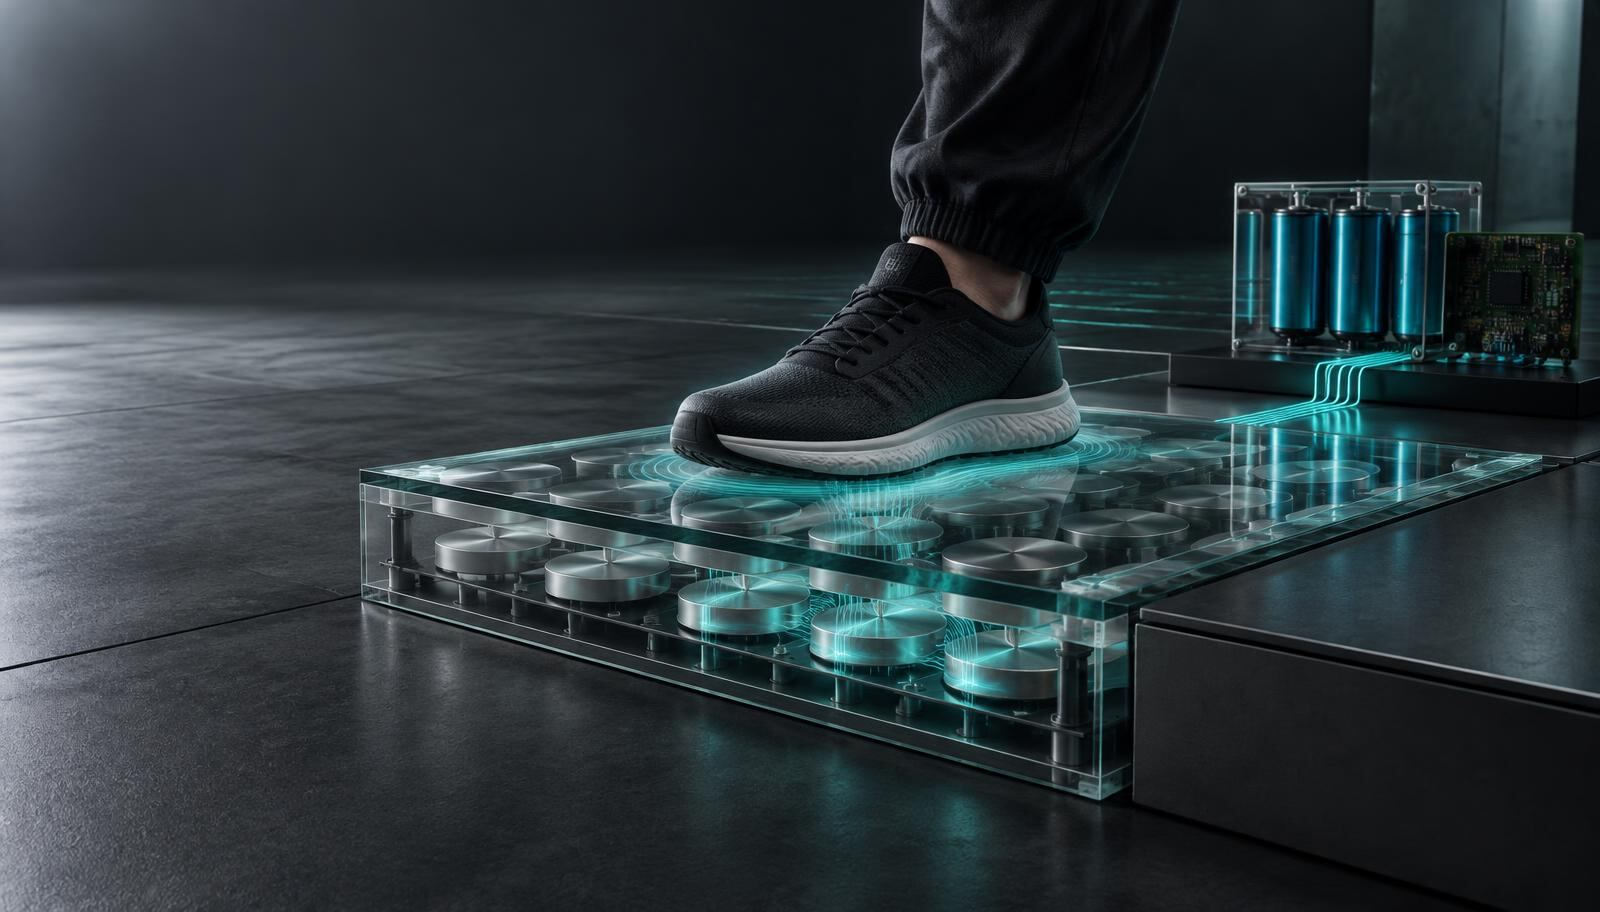
\includegraphics[width=0.88\textwidth,keepaspectratio]{figures/stepcharge-hero.jpg}
}{
    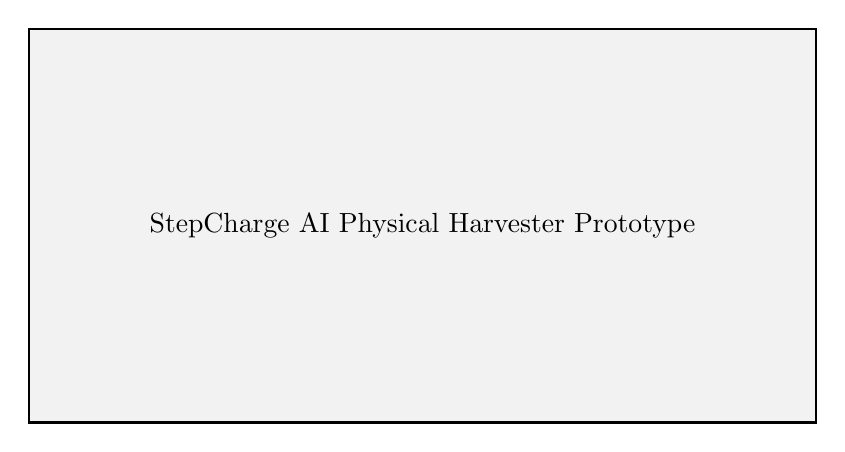
\begin{tikzpicture}
        \draw [thick, fill=gray!10] (0,0) rectangle (10,5) node[midway] {StepCharge AI Physical Harvester Prototype};
    \end{tikzpicture}
}
\caption{StepCharge AI physical footstep energy harvesting floor tile prototype.}
\label{fig:hero_prototype}
\end{figure}

\section{Hardware and Circuit Instrumentation}
Figure~\ref{fig:hardware_photo} illustrates the underlying piezoelectric transducer matrix, full-wave bridge rectification, supercapacitor buffer, and ESP32 microcontroller edge node.

\begin{figure}[H]
\centering
\IfFileExists{figures/visual-hardware.jpg}{
    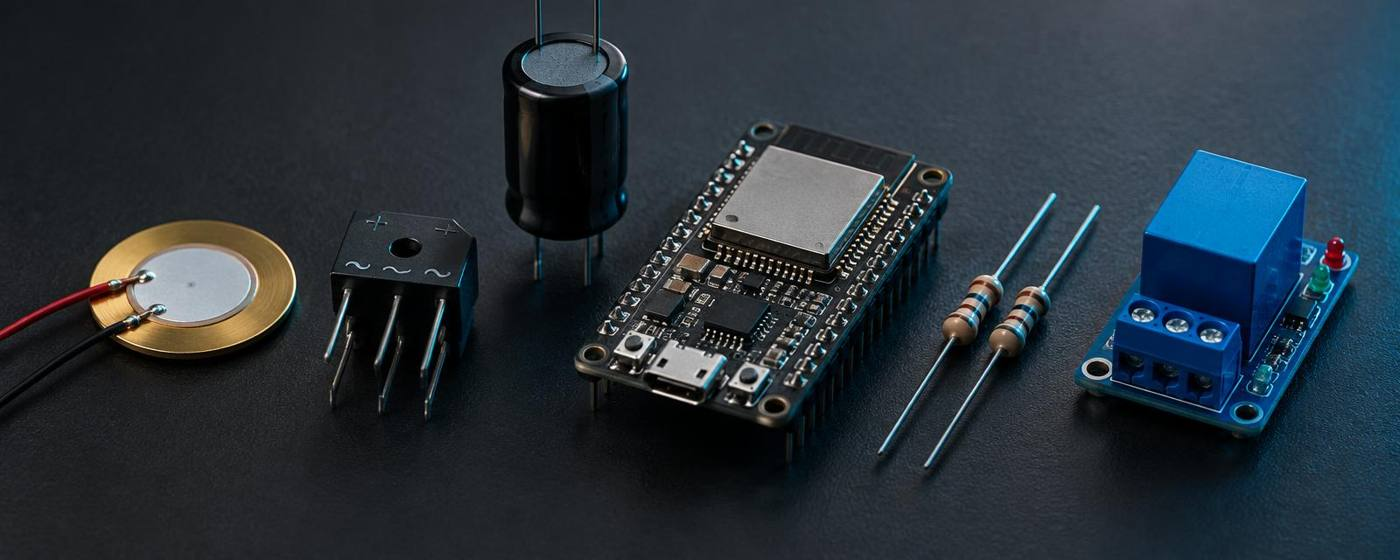
\includegraphics[width=0.85\textwidth,keepaspectratio]{figures/visual-hardware.jpg}
}{
    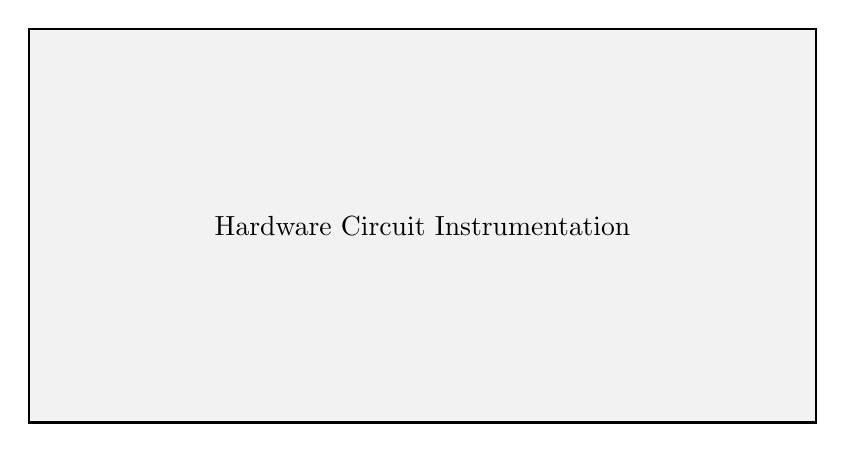
\begin{tikzpicture}
        \draw [thick, fill=gray!10] (0,0) rectangle (10,5) node[midway] {Hardware Circuit Instrumentation};
    \end{tikzpicture}
}
\caption{Internal hardware layout showing PZT transducer array and ESP32 conditioning circuitry.}
\label{fig:hardware_photo}
\end{figure}

\section{Real-Time Kinetic Energy Flow Monitoring}
Figure~\ref{fig:energy_flow_visual} shows the energy accumulation and real-time power management analytics visual rendered during continuous human walking trials.

\begin{figure}[H]
\centering
\IfFileExists{figures/visual-energy-flow.jpg}{
    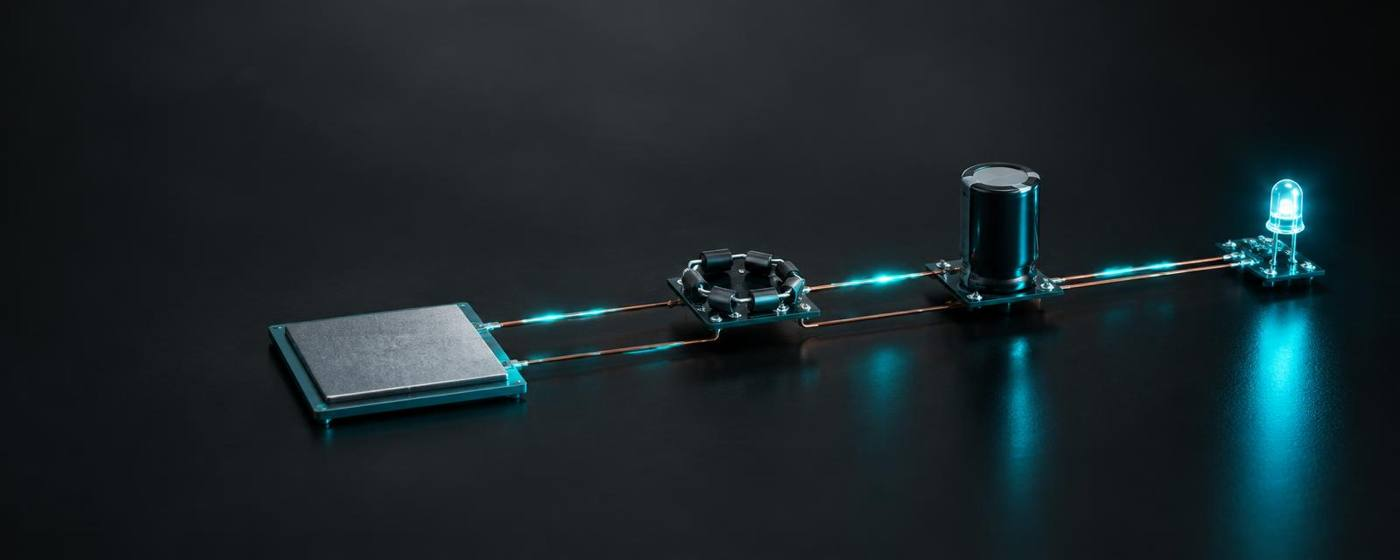
\includegraphics[width=0.85\textwidth,keepaspectratio]{figures/visual-energy-flow.jpg}
}{
    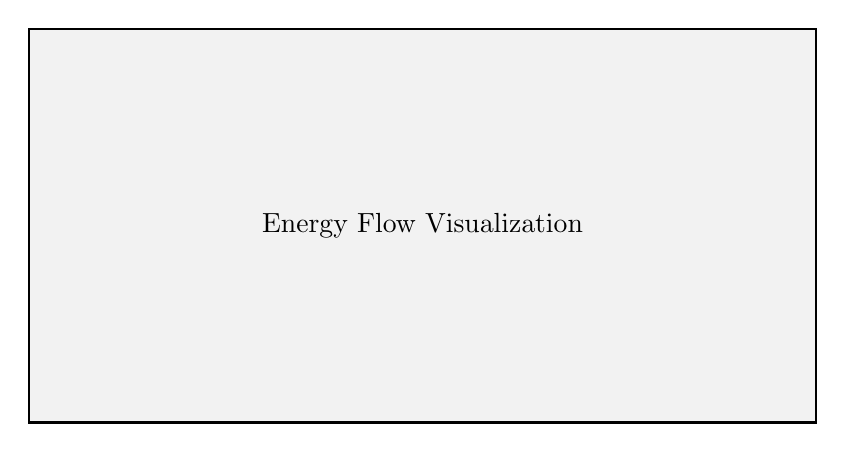
\begin{tikzpicture}
        \draw [thick, fill=gray!10] (0,0) rectangle (10,5) node[midway] {Energy Flow Visualization};
    \end{tikzpicture}
}
\caption{Real-time energy flow, voltage accumulation, and load management interface.}
\label{fig:energy_flow_visual}
\end{figure}

\section{Machine Learning Classification Visuals}
Figure~\ref{fig:ai_classification_visual} depicts the AI classification feed, presenting predicted gait intensity classes, confidence bars, and time-domain waveform feature extraction.

\begin{figure}[H]
\centering
\IfFileExists{figures/visual-ai-classification.jpg}{
    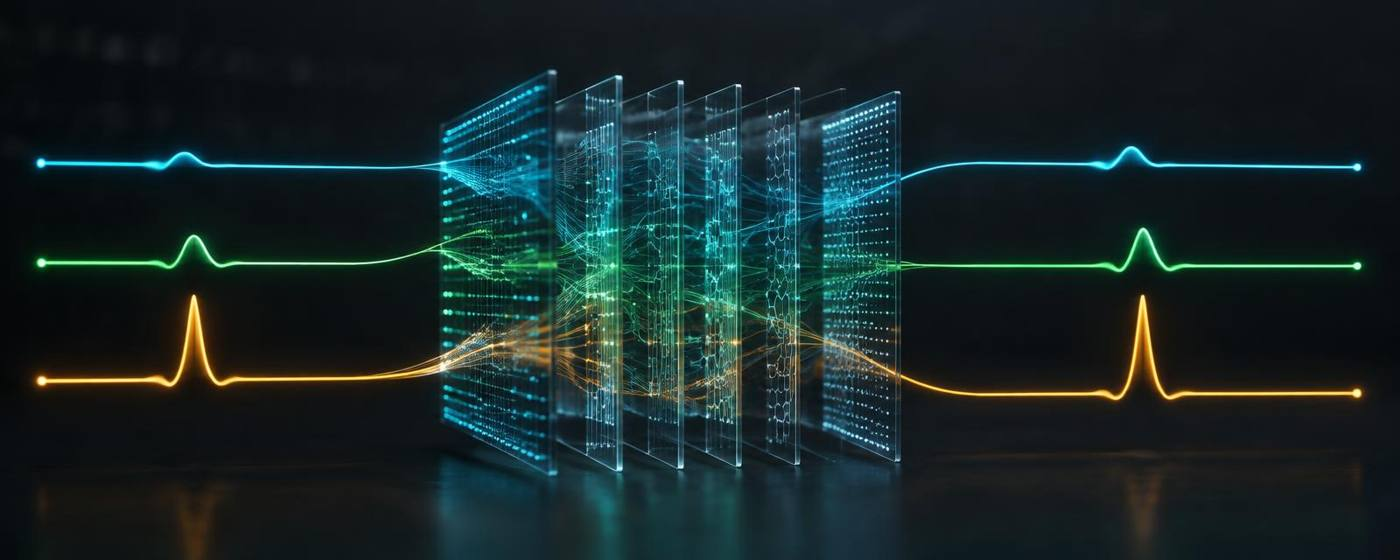
\includegraphics[width=0.85\textwidth,keepaspectratio]{figures/visual-ai-classification.jpg}
}{
    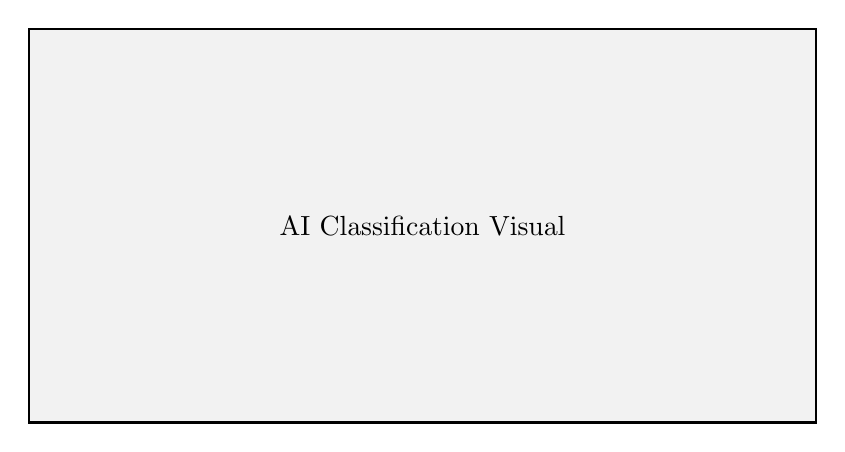
\begin{tikzpicture}
        \draw [thick, fill=gray!10] (0,0) rectangle (10,5) node[midway] {AI Classification Visual};
    \end{tikzpicture}
}
\caption{Machine learning footstep classification and kinetic intensity feed.}
\label{fig:ai_classification_visual}
\end{figure}

\section{IoT Network and Telemetry Architecture}
Figure~\ref{fig:iot_network_visual} displays the edge-to-cloud IoT telemetry network topology, showcasing secure device streaming and WebSocket distribution.

\begin{figure}[H]
\centering
\IfFileExists{figures/visual-iot-network.jpg}{
    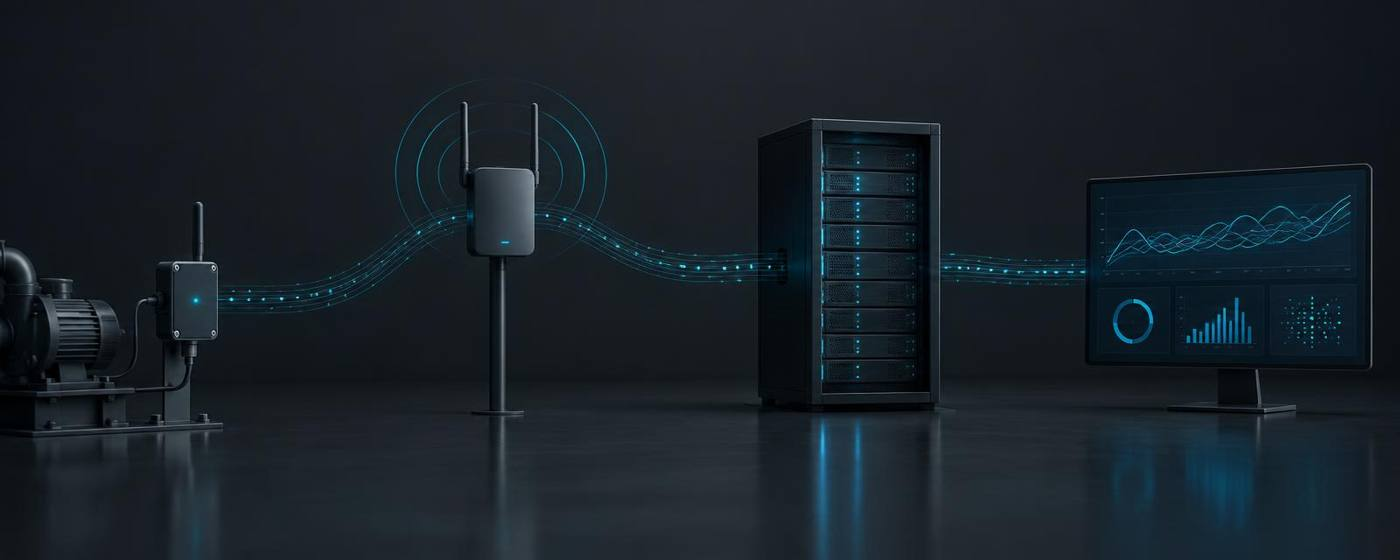
\includegraphics[width=0.85\textwidth,keepaspectratio]{figures/visual-iot-network.jpg}
}{
    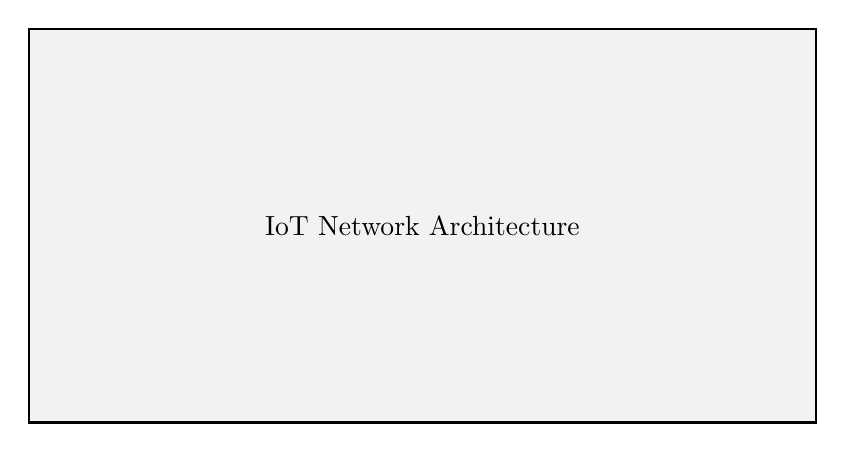
\begin{tikzpicture}
        \draw [thick, fill=gray!10] (0,0) rectangle (10,5) node[midway] {IoT Network Architecture};
    \end{tikzpicture}
}
\caption{IoT edge-to-cloud communication and real-time streaming pipeline.}
\label{fig:iot_network_visual}
\end{figure}
